\documentclass[oneside,a4paper,12pt]{article}
\usepackage{graphicx}
\usepackage[section]{placeins}
\usepackage{hyperref}
\graphicspath{{~/templates/}, {../images/anotated/}, {../images/}}

\makeindex
\begin{document}
	\begin{titlepage}
		\includegraphics[width=4cm]{logopopo.png}
		\hspace*{\fill}
		\includegraphics[width=6cm]{univlille.png}
		
		\begin{center}
			\vspace{1cm}
			\textbf{TP capteurs}\\
			\textbf{Commande d'un robot Pick and Place}\\
			\vspace{1cm}
			\textbf{Valentin DOSIAS, Maxence NEUS}\\
			\vspace{3cm}
			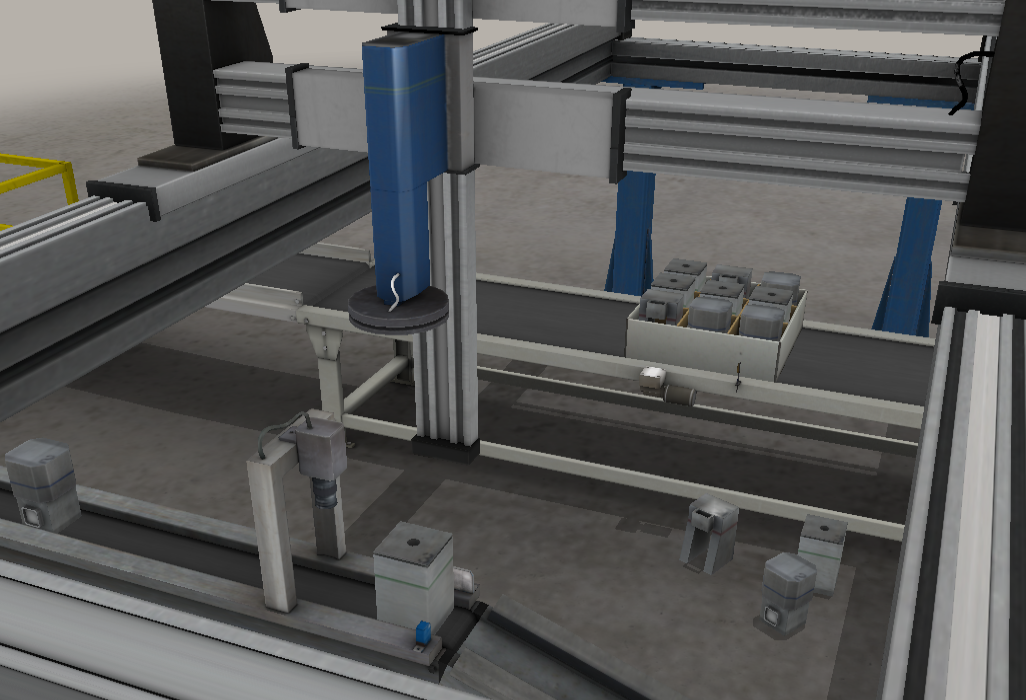
\includegraphics[width=13cm]{titlepage.PNG}\\
			\vspace{\fill}
			\textbf{Novembre 2021}\\
		\end{center}
	\end{titlepage}
	
	\tableofcontents
	\newpage
	
	\section{Introduction}
	
	Le TP consiste à concevoir et implémenter le système de commandes d’un robot Pick and place. La partie commande se fait via l’automate Schneider Modicon M340. La partie opérative est simulée sur l’ordinateur via un logiciel de simulation 3D appelé ITS PLC Professional Edition. Pour la commande du robot, nous utilisons des grafcets que nous concevons grâce au logiciel Unity Pro.  L’objectif de commande finale est de remplir totalement la caisse en ayant qu’un seul type de pièces par colonne. Lorsqu’une colonne est remplie, les pièces en trop doivent être évacuées. Pour ce faire nous avons d’abord pris en main le logiciel de simulation en activant nous-mêmes les différents actionneurs pour voir quel capteur est déclenché et à quel moment. Ensuite nous avons fait un programme pour que le robot mette une seule pièce par caisse. Une fois que la pièce est mise, la caisse est évacuée. Ensuite, nous avons modifié ce programme pour que la caisse soit remplie en entière et ensuite évacuée. Pour finir, nous avons ajouté la détection de chaque type de pièce pour remplir les colonnes en fonction du type de pièce.
	\newpage
	
	\section{Une pièce par boîte}
	
	Tout d’abord nous avons fait un grafcet pour prendre une pièce et le mettre dans la case (C0;L1). Une fois que la pièce est posée dans la caisse, la caisse peut-être évacuée. Nous avons donc conçu le grafcet suivant.\\
	
		\begin{figure}[h]
			\centering
			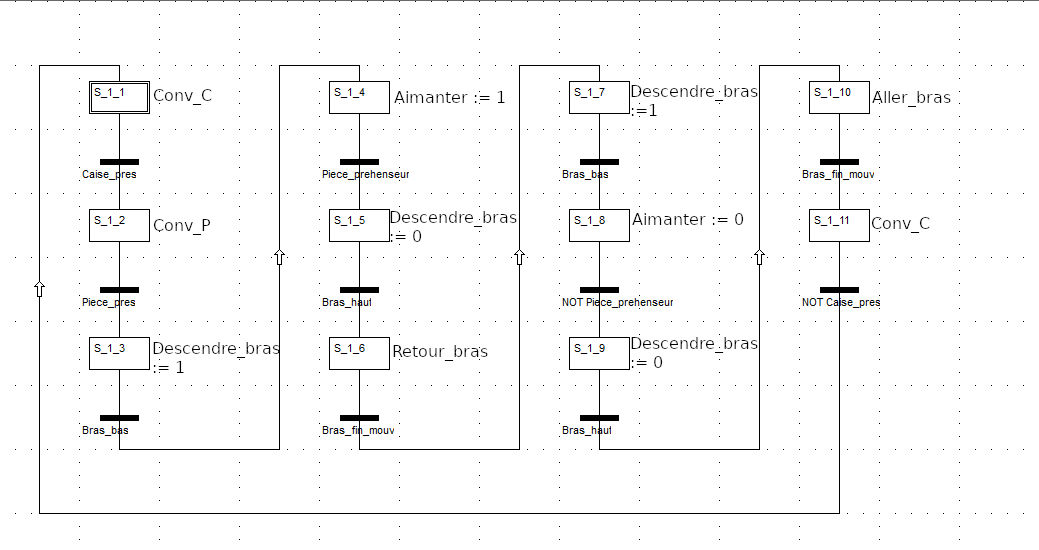
\includegraphics[width=15cm]{grafcet1.PNG}
			\caption{Une pièce par boîte}
		\end{figure}
	
	En premier lieu, nous attendons une caisse en activant le convoyeur des caisses (S\_1\_1 :Conv\_C). Une fois que la caisse est là, le convoyeur est automatiquement désactivé. Nous attendons ensuite une pièce donc nous activons ensuite le convoyeur pour les pièces (S\_1\_2 : Conv\_P). Une fois que la pièce est présente, le convoyeur est désactivé. Nous supposons dans tout le reste du TP que lorsque nous commençons notre programme, le bras est toujours dans sa position de repos soit en (C0;L0). La pièce étant là nous pouvons descendre le bras et le maintenir en bas tant que la pièce n’est pas prise par le préhenseur (Descendre\_Bras:=1). Ensuite nous prenons la pièce avec le préhenseur, il faut maintenir l’aimantation tant que le bras n’est pas arrivé à la position au-dessus de la caisse (aimanter := 1). Le bras ne doit pas se déplacer en position basse donc nous le remontons pour qu’il puisse aller jusqu'à la caisse (Descendre\_bras :=0). Ensuite nous faisons aller le bras jusqu’à la position (C0;L1) (Retour\_bras), nous descendons donc le bras (Descendre\_bras := 1) pour poser la pièce sans la lâcher de haut. Nous pouvons maintenant poser la pièce (Aimanter :=0), remonter le bras (Descendre\_bras := 0 ) et faire revenir le bras à sa position de repos en (C0;L0). Pour finir nous faisons partir la caisse, il faut donc attendre que le capteur de présence de pièce repasse à 0 (NOT Caise\_pres). Une fois la pièce évacuée le grafcet peut recommencer.
	
	\begin{figure}[h]
		\centering
		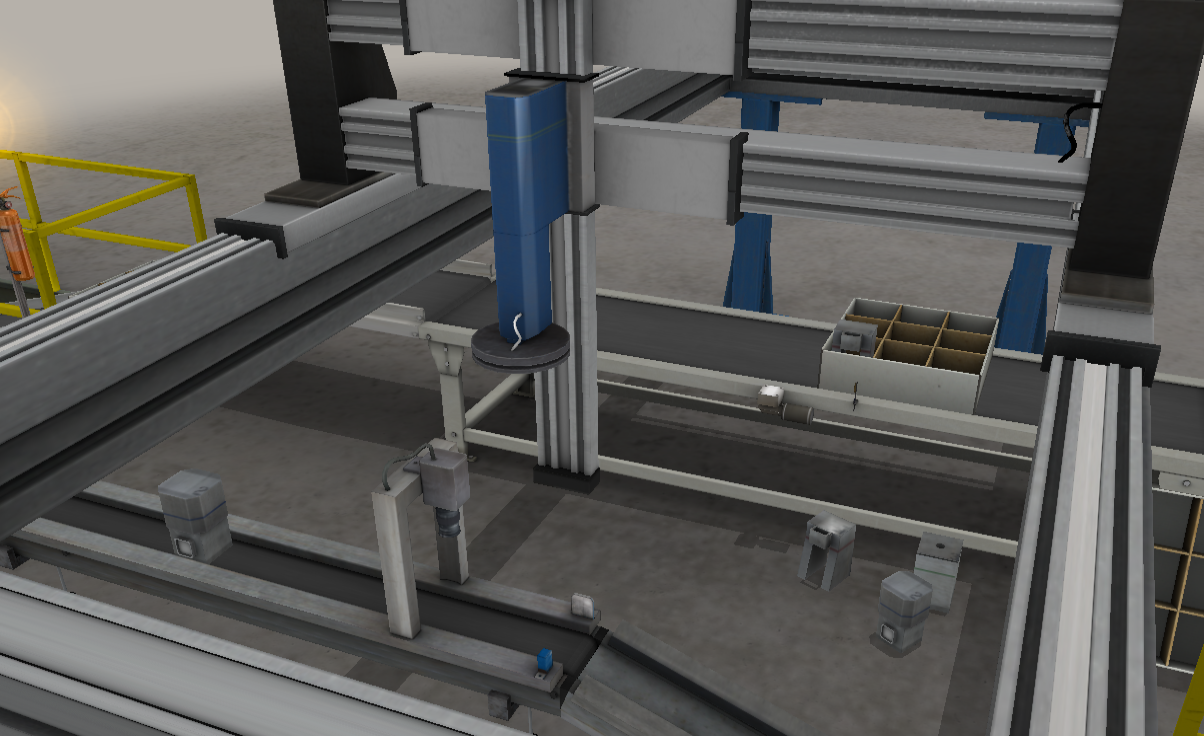
\includegraphics[width=12cm]{placementUnePiece.PNG}
		\caption{Une pièce par boîte}
	\end{figure}
	
	\section{Encapsulation des tâches de base}
	Pour ne pas avoir un grafcet général trop lourd, nous avons fait des macro-étapes pour les tâches de base pouvant être regroupées en une seule fonctionnalité.
	
		\paragraph{Préhensement}
		
		Nous avons réuni la tâche du préhenseur qui descend le bras saisit la pièce et remonte le bras dans la macro-étape Pick-Up.
	
		\paragraph{Dépose de pièce}
		
		La macro-étape Place va descendre le bras, poser la pièce et remonter le bras.
		
		\paragraph{Parallelisation}
		
		Nous avons trouvé un défaut à ce grafcet. Le défaut est qu’il faut attendre que la caisse soit bien présente pour envoyer une pièce, ce qui dans cette utilisation parait assez long. Nous avons donc choisi de gérer la présence des pièces avec un autre grafcet.
		
		\begin{figure}[h]
			\centering
			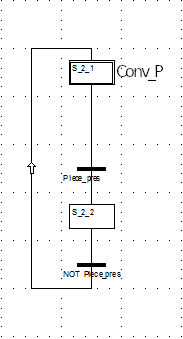
\includegraphics[width=5cm]{admission_pieces.PNG}
			\caption{Admission de pièces en parallele}
		\end{figure}
		
		Le grafcet est assez simple, nous activons le convoyeur, une fois que la pièce est arrivée, le convoyeur s’arrête et attend que la pièce ne soit plus présente, ce qui équivaut au préhenseur qui saisit la pièce. 
	
	\section{Remplissage d'une boîte}
				
		\subsection{Nouveau programme de déplacement}
			\paragraph{Logique de gestion des pièces}
			
			Pour éviter de faire 8 macro-étapes quasi identiques avec les différents cas de positionnement du bras à la position de la case ou de la position initiale, nous utilisons un compteur prenant des valeurs de 0 à 8. Pour chaque valeur est défini des valeurs pour le déplacement sur les lignes et sur les colonnes. Pour se rendre à la case, nous utilisons un certain nombre de fois les actionneurs Retour\_bras et Droite\_bras et pour le retour à la position initiale nous utilisons ce même nombre de fois les actionneurs Aller\_bras et Gauche\_bras.
			
			\paragraph{Algorithme de positionnement}

			Pour déplacer la pièce au bon endroit, nous utilisons les variables décrites dans la partie précédente. Nous les utilisons avec le grafcet suivant.
			
			\begin{figure}[h]
				\centering
				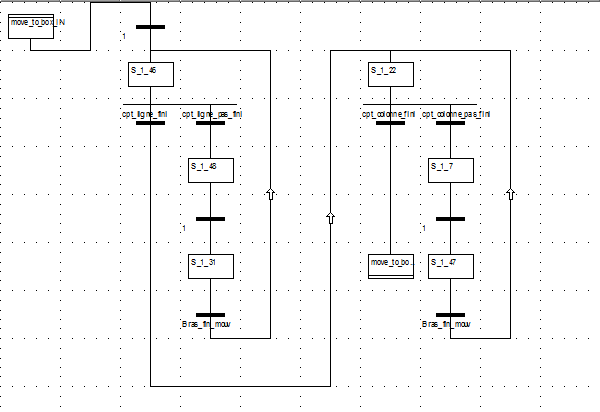
\includegraphics[width=12cm]{move_to_box.PNG}
				\caption{Algorithme de positionnement}
			\end{figure}
		
			Tout d’abord nous gérons les déplacements sur les lignes. Si les compteurs ont atteint la bonne valeur nous pouvons passer au déplacement sur les colonnes sinon nous faisons un déplacement sur la ligne en incrémentant le compteur. Nous faisons une pause de 3 secondes après le déplacement pour s’assurer que le capteur de fin de mouvement soit bien réinitialisé, ensuite nous vérifions que les valeurs du compteur et recommençons tant qu’il n’est pas arrivé à la bonne ligne. Pour les déplacements sur les colonnes le principe est le même. La macro-étape pour le retour à la position initiale est la même, seuls les actionneurs changent. Pour se rendre à la case, nous utilisons un certain nombre de fois les actionneurs Retour\_bras et Droite\_bras et pour le retour à la position initiale nous utilisons ce même nombre de fois les actionneurs Aller\_bras et Gauche\_bras.

	\section{Tri par type de pièce}
		\subsection{Nouvelle admission de pièces}
		
		\subsection{Ajustement du programme de déplacement}
	
	\section{Conclusion}
	
\end{document}
